
\documentclass{article}
\usepackage{graphicx} % Required for inserting images
\usepackage{hyperref}
\usepackage{caption} % For custom captions
\usepackage{amsmath}
\usepackage{multicol}

\title{Theoretical Mechanics: Big Homework 2}
\author{Ekaterina Mozhegova}
\date{March 13, 2024}

\begin{document}

\maketitle

\section{Link}
\href{https://github.com/illusoryTwin/Theoretical_mechanics/tree/master/hw7}{Link to the GitHub repository containing all the materials}
\href{https://colab.research.google.com/drive/1DiKK_ZvTILnPT2P7sJNKj1a4t78OqBTw?usp=sharing}{Colab}

\section{Task Description}
\begin{enumerate}
    \item Obtain the required measurements of the stand (like needed masses, lengths and so on).
    \item Gather the positions and velocities of the stand. You should run the same experiment 3 times each. 
    
    Initial conditions:
    \begin{itemize}
      \footnotesize
      \item $x = 0$, $\phi = 15^\circ$, $\dot{x} = 0$, $\dot{\phi} = 0$, $t=0$;
      \item $x = 0.25\ \text{m}$, $\phi = 45^\circ$, $\dot{x} = 0$, $\dot{\phi} = 0$, $t=0$;
      \item $x = 0.25\ \text{m}$, $\phi = -135^\circ$, $\dot{x} = 0$, $\dot{\phi} = 0$, $t=0$;
    \end{itemize}
    \item Substitute real data to your math model from HW 7, 8 (you can choose any method you like) and compare the results (propose and justify the metric).
    \item Explain what affects the difference between the math model and real data. Is the difference significant? 
    \item If so, change the model (add new forces, change the object representation), gather new needed data and compare it again.
    \item Make a conclusion.
\end{enumerate}

\subsection{What report should contain}
\begin{itemize}
\item The list of used tools and applications (I gathered a trajectory dataset using $x$ tool), etc.
\item The list of data you gathered from the stand and how did you do it.
\item Show how you conducted experiments. Is there any difference when you did the same experiment? Show it using plots and/or other metrics like $std,\ mse$ and so on.
\item Show the way how you chose the metrics for trajectory comparison, how you justify the answer.
\item If the error is too large, explain how you wanted to change your model and why you chose such a path.
\item Summarize your experience.
\end{itemize}

\section{Tools}
Python was used for data handling and solving dynamics.
Arduino was used for obtaining the data from the encoders of the stand.

\section{Methodology}

\subsection{Data retrieving}

To measure the state (position and velocity) of our system, we used the data from the encoders of the stand. 
Firstly, we changed the encoders tape to a new one since the suggested one provided us with noisy, inaccurate results.
In GitHub, you can find the Arduino script for reading the data from the encoders.

For both encoders, we measured the maximum range of values. Knowing the length of the rails 
(428 mm) and the maximum possible rotation angle of the rod ($360^\circ$), we can convert to the desired unit of measurement.

We conducted 3 experiments for each set of initial conditions and obtained datasets of 200 values for each experiment.

\begin{figure}[h]
  \centering
  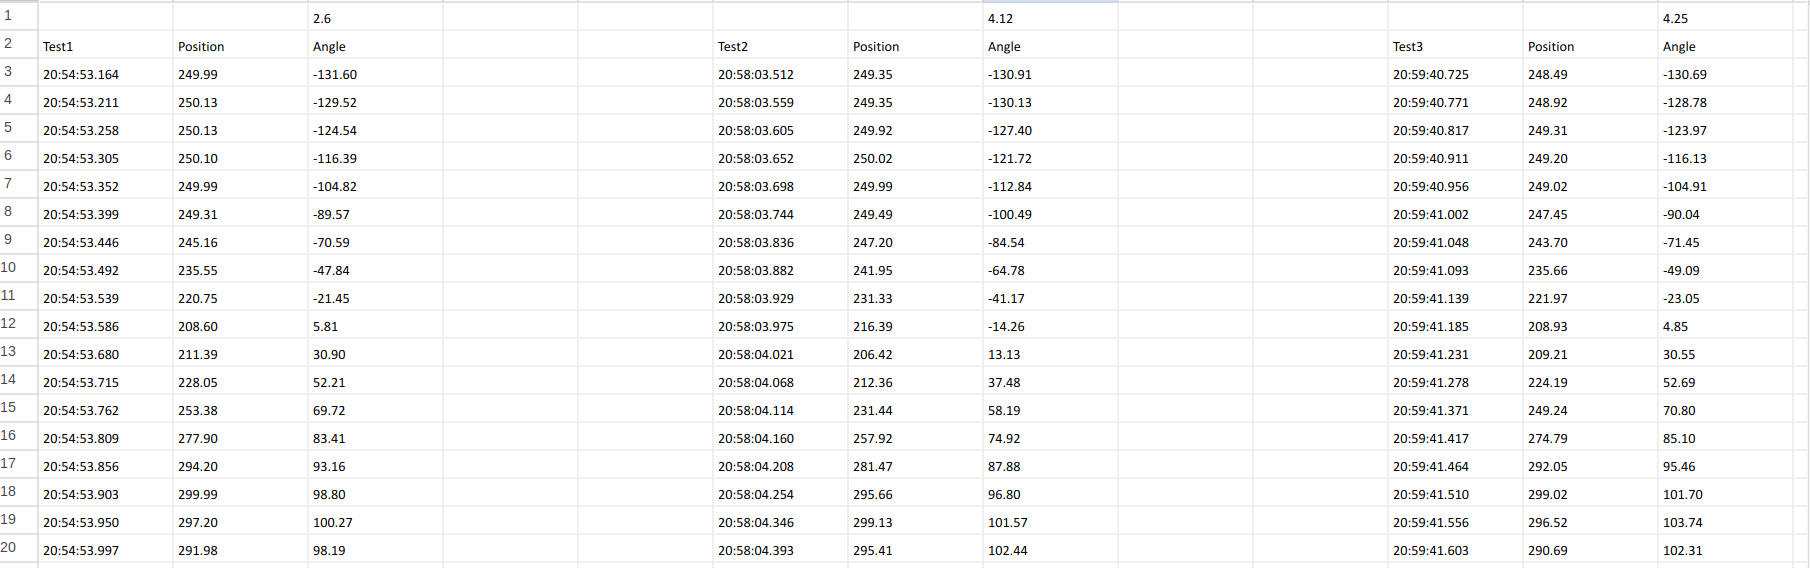
\includegraphics[scale=0.21]{data/measurements.png}
  \caption{Example: extract of the obtained data table}
\end{figure}

\subsection{Data visualization}
For each set of initial conditions, we calculated the mean value of the state (angle and position) from three experiments. 

The plotted values are as follows.\\

\textbf{Initial condition 1: $\phi = 10^\circ$, $x = 0$}

\includegraphics*[scale=0.7]{plots/init1!.png}

\textbf{Initial condition 2: $\phi = 45^\circ$, $x = 0.5$}

\includegraphics*[scale=0.7]{plots/init2!.png}\\\\


\textbf{Initial condition 3: $\phi = -135^\circ$, $x = 0.5$}

\includegraphics*[scale=0.8]{plots/init3!.png}

\section{Task Explanation. Analytical solution}

\textbf{Research object:} A system of 2 rods: rod 1 and rod 2\\
\textbf{Motion:} Rod 1 - rotational and plane motions, rod 2 - rotational and plane motions\\
\textbf{Force analysis:} $G_1 = m_1 g$, $G_2 = m_2 g$, $F_\text{fr}$, $F_\text{drag}$\\
\textbf{Solution:}

Let's solve the system using Newton-Euler method.

To accurately model the real-world system, it is necessary to incorporate air drag and friction into our dynamics equations.

\begin{align*}
  \text{eq1:} & \quad -T \sin(\phi) + m_1 \ddot{x} + k m_1 g \tanh(1000 \dot{x}) = 0 \\
  \text{eq2:} & \quad N - m_1 g - T \cos(\phi) = 0 \\
  \text{eq3:} & \quad T \sin(\phi) + m_2 \left(\ddot{\phi} \cdot l \cos(\phi) - \dot{\phi}^2 \cdot l \sin(\phi) + \ddot{x}\right) + k_{\text{air}} \sin(\phi) \tanh(1000 \dot{x}) = 0 \\
  \text{eq4:} & \quad T \cos(\phi) - m_2 g - m_2 \left(\ddot{\phi} \cdot l \sin(\phi) + \dot{\phi}^2 \cdot l \cos(\phi)\right) + k_{\text{air}} \cos(\phi) \tanh(1000 \dot{x}) = 0
\end{align*}
  
$F_\text{fr}$ changes the sign, and to handle it, we introduce $\tanh(1000 \dot{x})$.

Substitute constants (e.g., masses) with the values we measured.

\begin{enumerate}
  \item Mass of the rod's head - $154 \text{g}$.

  \item Mass of the cart - $266 \text{g}$.

  \item The mass of the rod, $11 \text{g}$, we can assume negligibly small.
\end{enumerate}

Take the average value of $k_\text{air}$ in indoor conditions similar to ours, $k_\text{air} = 0.5$ and $k = 0.2$.

Solve computationally with sympy.

\section{Plots}
\includegraphics*[scale=0.25]{plots/analytical_sol_plots.png}

\textbf{Initial condition 1: $\phi = 10^\circ$, $x = 0$}

\includegraphics*[scale=0.45]{plots/res_comparison_init1.png}

\newpage

\textbf{Initial condition 2: $\phi = 45^\circ$, $x = 0.25$}

\includegraphics*[scale=0.45]{plots/res_comparison_init2.png}


\textbf{Initial condition 3: $\phi = -135^\circ$, $x = 0.25$}

\includegraphics*[scale=0.45]{plots/res_comparison_init3.png}

\section{Discussion}

From the plots, we observe discrepancies in the positions of x, while $\phi$ is predicted quite accurately. Although we made assumptions and theoretical suggestions concerning the coefficients of friction and air resistance, their precise values are unknown to us. For more accurate results, determining these values is necessary. 

Additionally, in our experiment, we neglected the mass of the rod due to its relatively small value. However, for future, more accurate research, considering this mass might be reasonable.

Also, the issue with x might arise from high friction in the bearings, causing the cart to deviate slightly from its initial position. Determining this friction coefficient in practice is a non-trivial task, which could be a subject for further research.

\section{Team management:} Mikhail and I changed the tape in the cart-pole system to overcome the excessively high error. We connected an Arduino to it to obtain the required measurements of the stand. Timur, Leonid, Andrey, Elina, Reza, and I measured the values, while Mikhail and Yura solved the dynamics, data parsing - me.

\end{document}